\documentclass[11pt]{article}
\usepackage{goldsteinnotes}
\usepackage{tikz}
\usetikzlibrary{arrows.meta,calc,decorations.pathmorphing,decorations.markings,patterns,positioning,angles,quotes}

% --- document-specific symbol choices ---------------------------------------
% Euler angles as used throughout: alpha (azimuthal), beta (polar), gamma (spin
% about e3). Numbered body/inertial triads e1,e2,e3 and e1^0,e2^0,e3^0.
\newcommand{\ehat}[1]{\hat e_{#1}}
\newcommand{\ehatz}[1]{\hat e_{#1}^{0}}
\newcommand{\ebeta}{\hat e_{\beta}}
\newcommand{\Om}{\Omega}

\title{Rigid-Body Rotations}
\author{}
\date{}

\begin{document}
\maketitle
\vspace{-2.5em}

\section{Angular Momentum, Torque, and Energy for Rotation about a Fixed Axis}

For rotation about a fixed axis (the $z$-axis),
\begin{equation}
L_z = I\omega_z, \qquad \vec N = \vec P\times\vec F, \qquad T = \frac{I}{2}\omega_z^2 = \frac{\omega_z L_z}{2},
\label{eq:elem-1}
\end{equation}
where $\vec P$ is the position vector of the point of application of the force $\vec F$. The rate of change of angular momentum equals the external torque,
\begin{equation}
\ddt{\vec L} = \vec N^{(e)},
\label{eq:dLdt-Ne}
\end{equation}
evaluated either in an inertial frame, or in the center-of-mass (CM) frame (origin at the CM, axes parallel to the inertial axes).

\subsection{Rolling without Slipping}

For a wheel of radius $R$ rolling on a horizontal surface (Fig.~\ref{fig:rolling}), the rolling-without-slipping condition is
\begin{equation}
v_{\mathrm{CM}x} + \omega_z R = 0, \qquad (\omega_z<0 \text{ for clockwise rotation}).
\label{eq:rolling}
\end{equation}

\begin{figure}[htb]
\centering
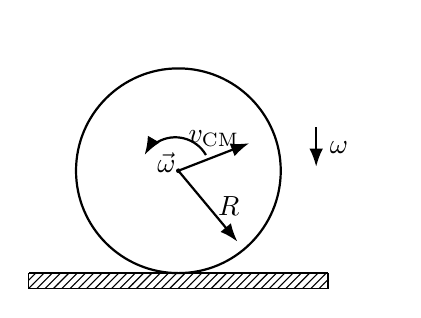
\begin{tikzpicture}[scale=1.0,>=Latex]
\draw[thick] (0,0) circle (1.3);
\fill (0,0) circle (0.03);
\draw[->,thick] (0,0) -- (0.9,0.35) node[midway,above] {$v_{\mathrm{CM}}$};
\draw[->,thick] (0,0) -- (0.75,-0.9) node[midway,right] {$R$};
\draw[->,thick] (0.35,0.2) arc (30:150:0.45);
\node at (-0.15,0.1) {$\vec\omega$};
\draw[->,thick] (1.75,0.55) -- (1.75,0.05);
\node[right] at (1.8,0.3) {$\omega$};
\draw[pattern=north east lines] (-1.9,-1.3) rectangle (1.9,-1.5);
\draw[thick] (-1.9,-1.3) -- (1.9,-1.3);
\node at (2.6,1.7) {};
\end{tikzpicture}
\hspace{1.3cm}
\begin{tikzpicture}[scale=1.0,>=Latex]
\draw[->,thick] (0,-0.3) -- (0,2.1) node[above] {$+y$};
\draw[->,thick] (-0.3,0) -- (2.4,0) node[right] {$+x$};
\end{tikzpicture}
\caption{Rolling without slipping: a wheel of radius $R$ with angular velocity $\vec\omega$ (clockwise for the sense drawn) and center-of-mass velocity $v_{\mathrm{CM}}$, resting on a fixed surface, together with the sign convention for the $x$-$y$ plane.}
\label{fig:rolling}
\end{figure}

\subsection{The Parallel-Axis Theorem (Elementary Form)}

For a rigid body rotating about a fixed axis a distance $a$ from the center of mass (Fig.~\ref{fig:parallel-elem}),
\begin{equation}
I = \bar I + Ma^2,
\label{eq:parallel-elem}
\end{equation}
where $\bar I$ is the moment of inertia about the parallel axis through the center of mass and $a$ is the distance between the axis of rotation and the center of mass.

\begin{figure}[htb]
\centering
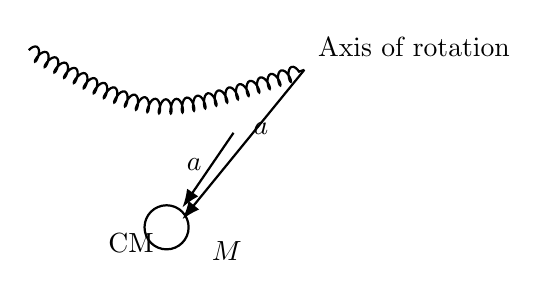
\begin{tikzpicture}[scale=1.0,>=Latex]
\draw[thick,decorate,decoration={coil,aspect=0.4,segment length=4}] (-1.6,1.6) .. controls (0,0.7) .. (1.9,1.35);
\draw[->,thick] (1.9,1.35) -- (0.35,-0.55) node[midway,above right] {$a$};
\draw[thick] (0.15,-0.65) circle (0.28);
\node[right] at (0.6,-0.95) {$M$};
\node[above right] at (1.95,1.4) {Axis of rotation};
\draw[->,thick] (1.0,0.55) -- (0.35,-0.4) node[midway,left] {};
\node at (0.5,0.15) {$a$};
\node at (-0.3,-0.85) {CM};
\end{tikzpicture}
\caption{The parallel-axis theorem: the axis of rotation lies a distance $a$ from the center of mass of an otherwise arbitrarily shaped rigid body.}
\label{fig:parallel-elem}
\end{figure}

\subsection{Separating the Center-of-Mass Motion}

For a system of particles with masses $m_j$ and positions $\vec r_j$, define the total mass, center-of-mass position, and positions relative to the center of mass:
\begin{equation}
M = \sum_j m_j, \qquad \vec R = \frac{\sum_j m_j\vec r_j}{M}, \qquad \vec r_j' \equiv \vec r_j - \vec R \quad (\text{position relative to CM}).
\label{eq:cm-defs}
\end{equation}
The total angular momentum and kinetic energy separate as
\begin{equation}
\vec L = \vec R\times M\dot{\vec R} + \sum_j \vec r_j'\times m_j\dot{\vec r}_j', \qquad
T = \frac{M}{2}\left|\dot{\vec R}\right|^2 + \frac12\sum_j m_j\left|\dot{\vec r}_j'\right|^2.
\label{eq:L-T-split}
\end{equation}
For a rigid body rotating with angular velocity $\omega_z$ about the CM,
\begin{equation}
L_z = \left(\vec R\times M\dot{\vec R}\right)_z + I\omega_z, \qquad T = \frac{M}{2}\left|\dot{\vec R}\right|^2 + \frac{I}{2}\omega_z^2.
\label{eq:L-T-rigid}
\end{equation}
Figure~\ref{fig:cm-vectors} shows the geometry: position vectors $\vec r_i$ from a fixed origin to each particle, the center-of-mass vector $\vec R$, and the relative vectors $\vec r_i'=\vec r_i-\vec R$.

\begin{figure}[htb]
\centering
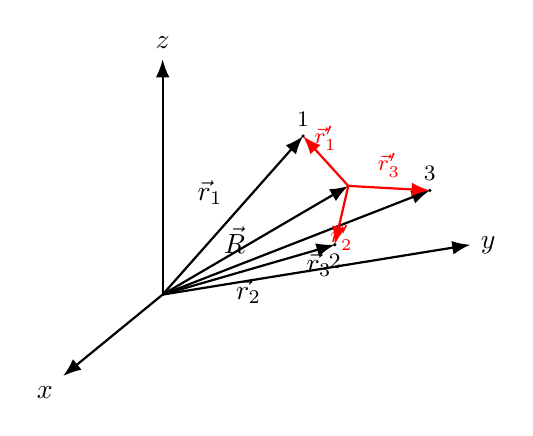
\begin{tikzpicture}[scale=1.15,>=Latex]
\draw[->,thick] (0,0) -- (0,2.6) node[above] {$z$};
\draw[->,thick] (0,0) -- (3.4,0.55) node[right] {$y$};
\draw[->,thick] (0,0) -- (-1.1,-0.9) node[below left] {$x$};
\coordinate (O) at (0,0);
\coordinate (P1) at (1.55,1.75);
\coordinate (P2) at (1.9,0.55);
\coordinate (P3) at (2.95,1.15);
\coordinate (R) at (2.05,1.2);
\draw[->,thick] (O) -- (P1) node[midway,above left] {$\vec r_1$};
\draw[->,thick] (O) -- (P2) node[midway,below] {$\vec r_2$};
\draw[->,thick] (O) -- (P3) node[midway,below right] {$\vec r_3$};
\draw[->,thick] (O) -- (R) node[midway,left] {$\vec R$};
\draw[->,red,thick] (R) -- (P1) node[midway,above] {\footnotesize $\vec r_1'$};
\draw[->,red,thick] (R) -- (P2) node[midway,below] {\footnotesize $\vec r_2'$};
\draw[->,red,thick] (R) -- (P3) node[midway,above] {\footnotesize $\vec r_3'$};
\fill (P1) circle (0.02); \fill (P2) circle (0.02); \fill (P3) circle (0.02);
\node[above] at (P1) {\footnotesize $1$};
\node[below] at (P2) {\footnotesize $2$};
\node[above] at (P3) {\footnotesize $3$};
\end{tikzpicture}
\caption{Position vectors $\vec r_i$ of individual particles measured from a fixed origin, the center-of-mass vector $\vec R$, and the vectors $\vec r_i'=\vec r_i-\vec R$ relative to the center of mass.}
\label{fig:cm-vectors}
\end{figure}

\subsubsection*{Proof}

Changing to the CM system, write $\vec r_i = \vec R+\vec r_i'$ and $\dot{\vec r}_i = \dot{\vec R}+\dot{\vec r}_i'$. Then
\begin{equation}
\vec L = \sum_{i=1}^N \vec r_i\times m_i\dot{\vec r}_i = \sum_{i=1}^N (\vec R+\vec r_i')\times m_i(\dot{\vec R}+\dot{\vec r}_i')
= \sum_i \vec R\times m_i\dot{\vec R} + \sum_i \vec r_i'\times m_i\dot{\vec r}_i' + \text{cross-terms}.
\label{eq:L-expand}
\end{equation}
The cross-terms vanish identically, using $M\vec R=\sum_i m_i\vec r_i$ and its time derivative (Newton's second law for the particle system, $M\ddot{\vec R}=\sum_i \vec F_i^{(e)}$, is not yet needed here):
\begin{align}
\sum_i \vec r_i'\times m_i\dot{\vec R} &= \sum_i m_i(\vec r_i-\vec R)\times\dot{\vec R} = \Big[\underbrace{\sum_i m_i\vec r_i}_{M\vec R} - \Big(\sum_i m_i\Big)\vec R\Big]\times\dot{\vec R} = \big[M\vec R - M\vec R\big]\times\dot{\vec R} = \vec 0,\\
\sum_i \vec R\times m_i\dot{\vec r}_i' &= \vec R\times\sum_i m_i(\dot{\vec r}_i-\dot{\vec R}) = \vec R\times\Big[\underbrace{\sum_i m_i\dot{\vec r}_i}_{M\dot{\vec R}} - \Big(\sum_i m_i\Big)\dot{\vec R}\Big] = \vec R\times\big[M\dot{\vec R}-M\dot{\vec R}\big] = \vec 0.
\end{align}
Hence
\begin{equation}
\vec L = \vec R\times M\dot{\vec R} + \sum_i \vec r_i'\times m_i\dot{\vec r}_i' \equiv \vec L^{(0)}, \qquad
\ddt{\vec L^{(0)}} = \vec R\times M\ddot{\vec R} + \sum_i \vec r_i'\times m_i\ddot{\vec r}_i'.
\label{eq:L0-def}
\end{equation}
But also, directly,
\begin{equation}
\ddt{\vec L^{(0)}} = \vec N^{(e)} = \sum_i \vec r_i\times \vec F_i^{(e)}, \qquad
\ddt{\vec L^{(0)}} = \vec R\times\sum_i \vec F_i^{(e)} + \sum_i \vec r_i'\times \vec F_i^{(e)} = \vec R\times M\ddot{\vec R}+\sum_i \vec r_i'\times \vec F_i^{(e)},
\label{eq:dL0-N}
\end{equation}
using $M\ddot{\vec R}=\sum_i \vec F_i^{(e)}$ (Newton's second law for the particle system). Comparing Eqs.~\eqref{eq:L0-def} and \eqref{eq:dL0-N}, the term $\vec R\times M\ddot{\vec R}$ cancels and
\begin{equation}
\ddt{\vec L'} = \sum_{i=1}^N \vec r_i'\times \vec F_i^{(e)}, \qquad \vec L'\equiv\sum_i \vec r_i'\times m_i\dot{\vec r}_i'.
\label{eq:dLprime}
\end{equation}
This is the special case of Eq.~\eqref{eq:dLdt-Ne} evaluated in the CM frame.

\section{Angular Velocity as an Antisymmetric Rotation-Rate Matrix}

For circular motion in a plane, $\vec v=\vec\omega\times\vec r$, with $\vec v\perp\vec r$ and $\vec v\cdot\vec r=0$. Let $\hat e_i$ ($i=1,2,3$) be an orthonormal, possibly time-dependent, basis:
\begin{equation}
\hat e_i\cdot\hat e_j = \delta_{ij} = \begin{cases}1 & i=j\\ 0 & i\neq j.\end{cases}
\label{eq:orthonormal}
\end{equation}
For a rotating coordinate system, differentiating $\delta_{ij}=\hat e_i\cdot\hat e_j$,
\begin{equation}
0 = \ddt{\delta_{ij}} = \ddt{}(\hat e_i\cdot\hat e_j) = \hat e_i\cdot\dd{\hat e_j}{t} + \hat e_j\cdot\dd{\hat e_i}{t}.
\label{eq:diff-delta}
\end{equation}
For $i=j$ this gives $0=\hat e_i\cdot \dd{\hat e_i}{t}$; for $i\neq j$ it gives $0=\hat e_i\cdot\dd{\hat e_j}{t}+\hat e_j\cdot\dd{\hat e_i}{t}$. Since $(\hat e_j)_{j=1,2,3}$ is a basis, $\dd{\hat e_i}{t}$ can be written as a linear combination of the $\hat e_j$:
\begin{equation}
\boxed{\dd{\hat e_i}{t} = \sum_{j=1}^3 \Om_{ij}\hat e_j, \qquad \Om_{ij}\equiv \hat e_j\cdot\dd{\hat e_i}{t},}
\label{eq:Omega-def}
\end{equation}
using that $\hat e_j\cdot\sum_i \sigma_i\hat e_i = \sum_i\sigma_i\hat e_j\cdot\hat e_i=\sigma_j$. From Eq.~\eqref{eq:diff-delta}, for $i\neq j$, $0=\Om_{ij}+\Om_{ji}\Rightarrow \Om_{ji}=-\Om_{ij}$, and $\Om_{ii}=\hat e_i\cdot\dd{\hat e_i}{t}=0$; that is, $\Om_{ij}$ is antisymmetric,
\begin{equation}
\Om = \begin{pmatrix} 0 & \Om_{12} & -\Om_{31}\\ -\Om_{12} & 0 & \Om_{23}\\ \Om_{31} & -\Om_{23} & 0\end{pmatrix}.
\label{eq:Omega-matrix}
\end{equation}
An antisymmetric $3\times3$ matrix has three independent entries, matched to the components of an axial vector $\vec\omega$ by
\begin{equation}
\omega_1\equiv\Om_{23}, \qquad \omega_2\equiv\Om_{31}, \qquad \omega_3\equiv\Om_{12}.
\label{eq:omega-axial}
\end{equation}
Explicitly,
\begin{align}
\dd{\hat e_1}{t} &= \Om_{12}\hat e_2+\Om_{13}\hat e_3 = \Om_{12}\hat e_2-\Om_{31}\hat e_3 = \omega_3\hat e_2-\omega_2\hat e_3 = \vec\omega\times\hat e_1,\label{eq:de1dt}\\
\dd{\hat e_2}{t} &= \Om_{21}\hat e_1+\Om_{23}\hat e_3 = -\Om_{12}\hat e_1+\Om_{23}\hat e_3 = -\omega_3\hat e_1+\omega_1\hat e_3 = \vec\omega\times\hat e_2,\label{eq:de2dt}\\
\dd{\hat e_3}{t} &= \vec\omega\times\hat e_3,\label{eq:de3dt}
\end{align}
where Eq.~\eqref{eq:de1dt} is checked directly: $\vec\omega\times\hat e_1=(\omega_1\hat e_1+\omega_2\hat e_2+\omega_3\hat e_3)\times\hat e_1=-\omega_2\hat e_3+\omega_3\hat e_2$, matching the left side; similarly for Eq.~\eqref{eq:de2dt}, using $\hat e_1\times\hat e_2=\hat e_3$ and $\hat e_3\times\hat e_2=-\hat e_1$.

\subsection{The Levi-Civita Symbol and Cross Products}

With $\hat e_1\equiv\hat x$, $\hat e_2\equiv\hat y$, $\hat e_3\equiv\hat z$ (Fig.~\ref{fig:triad}), so that $\hat e_1\times\hat e_2=\hat e_3$ (and cyclically), $\hat e_2\times\hat e_3=\hat e_1$, $\hat e_3\times\hat e_1=\hat e_2$, the Levi-Civita symbol is
\begin{equation}
\epsilon_{ijk} = \begin{cases}
+1 & ijk \text{ a cyclic permutation of } 123\\
-1 & ijk \text{ a cyclic permutation of } 213\\
0 & \text{if any index is repeated,}
\end{cases}
\label{eq:levicivita}
\end{equation}
so that $\epsilon_{123}=\epsilon_{231}=\epsilon_{312}=+1$, $\epsilon_{213}=\epsilon_{132}=\epsilon_{321}=-1$, $\epsilon_{iij}=\epsilon_{iji}=\epsilon_{jii}=0$, and
\begin{equation}
\hat e_i\times\hat e_j = \sum_\ell \epsilon_{ij\ell}\,\hat e_\ell.
\label{eq:eixej}
\end{equation}

\begin{figure}[htb]
\centering
\begin{tikzpicture}[scale=1.1,>=Latex]
\draw[->,thick] (0,0) -- (0,1.5) node[above] {$\hat z$};
\draw[->,thick] (0,0) -- (1.5,0) node[right] {$\hat y$};
\draw[->,thick] (0,0) -- (-1.0,-0.75) node[below left] {$\hat x$};
\draw[thick] (0,0) circle (0.06);
\end{tikzpicture}
\caption{Right-handed orthonormal triad used for the Levi-Civita convention: $\hat x\times\hat y=\hat z$ and cyclically.}
\label{fig:triad}
\end{figure}

\section{The Transport Theorem for Rotating Frames}

Let $\hat e_1^0,\hat e_2^0,\hat e_3^0$ be a fixed inertial triad and $\hat e_1,\hat e_2,\hat e_3$ a rotating (non-inertial) triad (Fig.~\ref{fig:frames}). For an arbitrary vector $\vec b(t)$ with components $b_i^0$ in the inertial basis and $b_i$ in the rotating basis,
\begin{equation}
\left.\ddt{\vec b}\right|_{\mathrm{inertial}} = \ddt{}\left(\sum_{i=1}^3 b_i^0\hat e_i^0\right) = \sum_{i=1}^3 \dot b_i^0\hat e_i^0, \qquad
\left.\ddt{\vec b}\right|_{\mathrm{body}} \equiv \sum_{i=1}^3 \dd{b_i}{t}\hat e_i,
\label{eq:body-deriv-def}
\end{equation}
while resolving $\vec b$ in the rotating basis and differentiating in the inertial frame,
\begin{equation}
\left.\ddt{\vec b}\right|_{\mathrm{inertial}} = \ddt{}\left(\sum_{i=1}^3 b_i\hat e_i\right) = \sum_{i=1}^3 \dot b_i\hat e_i + \sum_{i=1}^3 b_i\dot{\hat e}_i.
\label{eq:body-deriv-expand}
\end{equation}
Using $\dot{\hat e}_i=\vec\omega\times\hat e_i$ (Eq.~\eqref{eq:de1dt}),
\begin{equation}
\left.\ddt{\vec b}\right|_{\mathrm{inertial}} = \left.\ddt{\vec b}\right|_{\mathrm{body}} + \sum_{i=1}^3 b_i(\vec\omega\times\hat e_i),
\label{eq:transport-sum}
\end{equation}
so that
\begin{equation}
\boxed{\left.\ddt{\vec b}\right|_{\mathrm{inertial}} = \left.\ddt{\vec b}\right|_{\mathrm{body}} + \vec\omega\times\vec b.}
\label{eq:transport}
\end{equation}

\begin{figure}[htb]
\centering
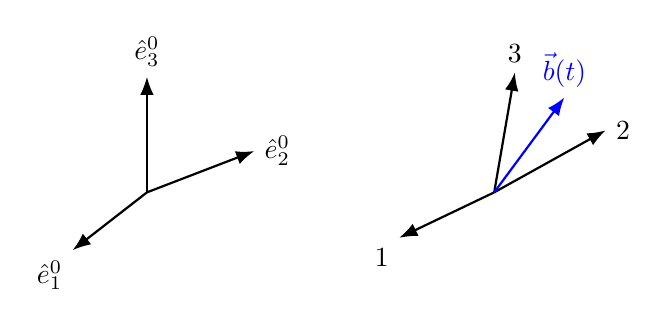
\begin{tikzpicture}[scale=1.05,>=Latex]
\draw[->,thick] (0,0) -- (0,1.4) node[above] {$\hat e_3^0$};
\draw[->,thick] (0,0) -- (1.3,0.5) node[right] {$\hat e_2^0$};
\draw[->,thick] (0,0) -- (-0.9,-0.7) node[below left] {$\hat e_1^0$};
\begin{scope}[xshift=4.2cm]
\draw[->,thick] (0,0) -- (0.25,1.45) node[above] {$3$};
\draw[->,thick] (0,0) -- (1.35,0.75) node[right] {$2$};
\draw[->,thick] (0,0) -- (-1.15,-0.55) node[below left] {$1$};
\draw[->,thick,blue] (0,0) -- (0.85,1.15) node[above,blue] {$\vec b(t)$};
\end{scope}
\end{tikzpicture}
\caption{Fixed inertial triad $\hat e_1^0,\hat e_2^0,\hat e_3^0$ (left) and rotating body triad $\hat e_1,\hat e_2,\hat e_3$ (right, labeled $1,2,3$), together with an arbitrary vector $\vec b(t)$ resolved in the rotating basis.}
\label{fig:frames}
\end{figure}

\subsection{Rigid-Body Kinetic Energy from the Transport Theorem}

For a rigid body with a fixed point, let $\vec r_P$ be the (constant, in the body frame) position of point $P$ in the body frame. Since the body is rigid, $\vec v_P=\vec\omega\times\vec r_P$, and
\begin{equation}
T = \sum_P \frac12 m_P v_P^2 = \sum_P \frac12 m_P\left(\vec\omega\times\vec r_P\right)^2.
\label{eq:T-rigid-fixed}
\end{equation}
Useful vector identities, verified using the Levi-Civita symbol:
\begin{equation}
\hat e_1\times\hat e_2=\hat e_3=\sum_\ell\epsilon_{12\ell}\hat e_\ell, \qquad
\vec a\times\vec b = \Big(\sum_i a_i\hat e_i\Big)\times\Big(\sum_j b_j\hat e_j\Big) = \sum_{ij\ell}a_ib_j\epsilon_{ij\ell}\hat e_\ell,
\label{eq:axb-component}
\end{equation}
\begin{equation}
(\vec a\times\vec b)_k=\sum_{ij}\epsilon_{ijk}a_ib_j,
\label{eq:axb-component-k}
\end{equation}
and, using $\sum_i \epsilon_{jki}\epsilon_{\ell mi}=\delta_{j\ell}\delta_{km}-\delta_{jm}\delta_{k\ell}$ together with the cyclic property $\epsilon_{ijk}=\epsilon_{jki}=\epsilon_{kij}$,
\begin{align}
(\vec A\times\vec B)\cdot(\vec C\times\vec D) &= \sum_{ijk}A_iB_j\epsilon_{ijk}\hat e_k \cdot \sum_{\ell m n}C_\ell D_m\epsilon_{\ell mn}\hat e_n
= \sum_{ijk\ell m}\epsilon_{ijk}\epsilon_{\ell mk}A_iB_jC_\ell D_m\notag\\
&= (\vec A\cdot\vec C)(\vec B\cdot\vec D)-(\vec A\cdot\vec D)(\vec B\cdot\vec C).
\label{eq:bac-cab}
\end{align}

\section{Rigid-Body Kinetic Energy and the Inertia Tensor}

Applying Eq.~\eqref{eq:bac-cab} to Eq.~\eqref{eq:T-rigid-fixed} with $\vec A=\vec C=\vec\omega$, $\vec B=\vec D=\vec r_P$,
\begin{equation}
T = \sum_P\frac{m_P}{2}\Big[\omega^2 r_P^2-(\vec\omega\cdot\vec r_P)^2\Big].
\label{eq:T-expand1}
\end{equation}
Writing this in components,
\begin{equation}
T = \frac12\sum_P m_P\left[r_P^2\sum_{i=1}^3\omega_i\omega_i - \Big(\sum_{i=1}^3\omega_ir_{Pi}\Big)\Big(\sum_{j=1}^3\omega_jr_{Pj}\Big)\right]
= \frac12\sum_P m_P\sum_{ij=1}^3\Big[r_P^2\delta_{ij}-r_{Pi}r_{Pj}\Big]\omega_i\omega_j,
\label{eq:T-component}
\end{equation}
so that
\begin{equation}
\boxed{T = \frac12\sum_{ij=1}^3 I_{ij}\,\omega_i\omega_j,} \qquad
\boxed{I_{ij}\equiv\sum_P m_P\Big[r_P^2\delta_{ij}-r_{Pi}r_{Pj}\Big]} \quad \text{(moment of inertia tensor, symmetric).}
\label{eq:inertia-tensor-def}
\end{equation}
Likewise for the angular momentum,
\begin{equation}
\vec L = \sum_P m_P\,\vec r_P\times\vec v_P = \sum_P m_P\,\vec r_P\times(\vec\omega\times\vec r_P).
\label{eq:L-rigid}
\end{equation}

\subsection*{Aside: Summation-Notation Identity}

Using the epsilon-contraction identity of Eq.~\eqref{eq:bac-cab} in component form,
\begin{align}
\big[\vec A\times(\vec B\times\vec C)\big]_i &= \epsilon_{ijk}A_j\epsilon_{k\ell m}B_\ell C_m = \epsilon_{kij}\epsilon_{k\ell m}A_jB_\ell C_m\notag\\
&= (\delta_{i\ell}\delta_{jm}-\delta_{im}\delta_{j\ell})A_jB_\ell C_m = (\vec A\cdot\vec C)B_i - (\vec A\cdot\vec B)C_i,
\label{eq:aside-bac-cab}
\end{align}
using $\epsilon_{ijk}=\epsilon_{kij}$. Applying this to $\vec r_P\times(\vec\omega\times\vec r_P)$ with $\vec A=\vec B=\vec r_P$, $\vec C=\vec\omega$,
\begin{equation}
\big[\vec r_P\times(\vec\omega\times\vec r_P)\big]_i = (\vec r_P\cdot\vec r_P)\omega_i - (\vec r_P\cdot\vec\omega)r_{Pi},
\label{eq:rxwr}
\end{equation}
so that
\begin{equation}
L_i = \sum_P m_P\big[\vec r_P\times(\vec\omega\times\vec r_P)\big]_i = \sum_P m_P\left[r_P^2\omega_i - \sum_{j=1}^3 r_{Pi}r_{Pj}\omega_j\right]
= \sum_{j=1}^3\underbrace{\left(\sum_P m_P\big[r_P^2\delta_{ij}-r_{Pi}r_{Pj}\big]\right)}_{=I_{ij}}\omega_j.
\label{eq:Li-derivation}
\end{equation}
Collecting results,
\begin{equation}
\boxed{L_i = \sum_j I_{ij}\,\omega_j,} \qquad \boxed{T = \frac12\,\vec\omega\cdot\vec L,} \qquad \boxed{T = \frac12\sum_{ij=1}^3 I_{ij}\,\omega_i\omega_j.}
\label{eq:L-T-boxed}
\end{equation}

\section{Principal Axes}

Since $I_{ij}=I_{ji}=I_{ji}^*$, the inertia tensor is Hermitian (here, real symmetric) and can therefore be diagonalized:
\begin{equation}
I_{ij} = I_{ji} = I_{ji}^* \;\Rightarrow\; \text{Hermitian} \;\Rightarrow\; \text{diagonalizable}, \qquad
\begin{pmatrix} I_1 & 0 & 0\\ 0 & I_2 & 0\\ 0 & 0 & I_3\end{pmatrix}.
\label{eq:hermitian}
\end{equation}
The directions that diagonalize $I_{ij}$ are called the \emph{principal axes}.

\subsection{Examples}

For a homogeneous cube or sphere, all three principal moments coincide, $I_{ij}=I\delta_{ij}$, i.e.\ $\mathrm{diag}(I,I,I)=I\mathbf{1}_{3\times3}$. For an oblate body (radius $b$ much larger than the half-thickness $a$, Fig.~\ref{fig:principal-examples}a), $I_1=I_2>I_3$; for a prolate body (half-length $a$ much larger than the radius $b$, Fig.~\ref{fig:principal-examples}b), $I_1=I_2<I_3$. In general, for an irregular body, $I_1,I_2,I_3$ are all different.

\begin{figure}[htb]
\centering
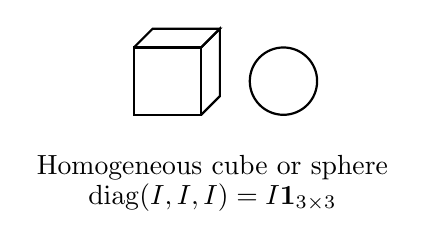
\begin{tikzpicture}[scale=0.95,>=Latex]
\draw[thick] (-2.6,0.55) rectangle (-1.7,1.45);
\draw[thick] (-2.6,1.45) -- (-2.35,1.7) -- (-1.45,1.7) -- (-1.7,1.45);
\draw[thick] (-1.7,1.45) -- (-1.45,1.7) -- (-1.45,0.8) -- (-1.7,0.55);
\draw[thick] (-0.6,1.0) circle (0.45);
\node at (-1.55,-0.15) {Homogeneous cube or sphere};
\node at (-1.55,-0.55) {$\mathrm{diag}(I,I,I)=I\mathbf{1}_{3\times3}$};
\end{tikzpicture}
\hspace{0.4cm}
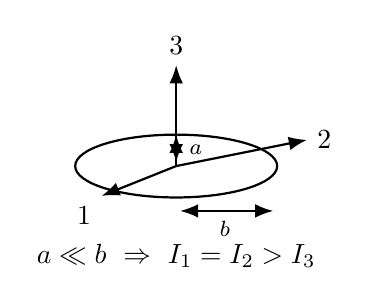
\begin{tikzpicture}[scale=0.95,>=Latex]
\draw[thick] (0,0) ellipse (1.35 and 0.42);
\draw[->,thick] (0,0) -- (0,1.35) node[above] {$3$};
\draw[->,thick] (0,0) -- (1.75,0.35) node[right] {$2$};
\draw[->,thick] (0,0) -- (-1.0,-0.4) node[below left] {$1$};
\draw[<->,thick] (0,0.05) -- (0,0.42);
\node[right] at (0.05,0.22) {\footnotesize $a$};
\draw[<->,thick] (0.05,-0.6) -- (1.3,-0.6);
\node[below] at (0.65,-0.6) {\footnotesize $b$};
\node at (0,-1.2) {$a\ll b\ \Rightarrow\ I_1=I_2>I_3$};
\end{tikzpicture}
\hspace{0.4cm}
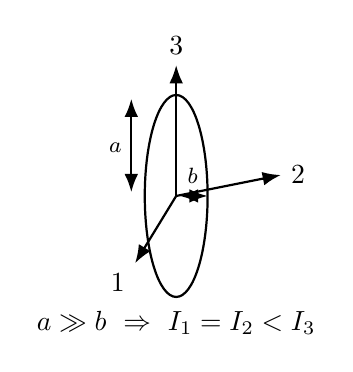
\begin{tikzpicture}[scale=0.95,>=Latex]
\draw[thick] (0,0) ellipse (0.42 and 1.35);
\draw[->,thick] (0,0) -- (0,1.75) node[above] {$3$};
\draw[->,thick] (0,0) -- (1.4,0.28) node[right] {$2$};
\draw[->,thick] (0,0) -- (-0.55,-0.9) node[below left] {$1$};
\draw[<->,thick] (0.05,0) -- (0.42,0);
\node[above] at (0.22,0.03) {\footnotesize $b$};
\draw[<->,thick] (-0.6,0.05) -- (-0.6,1.3);
\node[left] at (-0.6,0.65) {\footnotesize $a$};
\node at (0,-1.7) {$a\gg b\ \Rightarrow\ I_1=I_2<I_3$};
\end{tikzpicture}
\caption{Principal-axis examples: (left) a homogeneous cube or sphere, for which all principal moments coincide; (center) an oblate disk, $a\ll b$; (right) a prolate rod, $a\gg b$.}
\label{fig:principal-examples}
\end{figure}

These follow from $I=\sum_P m_P(\text{distance to axis})^2=\sum_P m_P r_{P1}^2$ for rotation about axis $1$: since $r_{P1}r_{P1}+r_{P2}r_{P2}+r_{P3}r_{P3}-r_{P3}r_{P3}=r_{P1}^2$, i.e.\ $x^2+y^2+z^2-z^2=x^2+y^2\equiv\rho^2$ for the axis $3$ (using $I_{33}=\sum_P m_P[\delta_{33}r_P^2-r_{P3}r_{P3}]$), one has $I_3\sim Ma^2$, $I_1\sim Mb^2$: if $a\ll b$ then $I_3\ll I_1$, and if $a\gg b$ then $I_3\gg I_1$.

\subsection{Diagonal Form}

In the principal-axis basis, $I_{ij}=I_i\delta_{ij}$, and
\begin{equation}
L_i = \sum_{j=1}^3 I_{ij}\omega_j = \sum_{j=1}^3 I_i\delta_{ij}\omega_j = I_i\omega_i, \qquad
\begin{pmatrix}L_1\\L_2\\L_3\end{pmatrix} = \begin{pmatrix}I_1&0&0\\0&I_2&0\\0&0&I_3\end{pmatrix}\begin{pmatrix}\omega_1\\\omega_2\\\omega_3\end{pmatrix} = \begin{pmatrix}I_1\omega_1\\I_2\omega_2\\I_3\omega_3\end{pmatrix},
\label{eq:diag-L}
\end{equation}
\begin{equation}
T = \frac12\vec\omega\cdot\vec L = \frac12\sum_{i=1}^3\omega_iL_i = \frac12\sum_{i=1}^3\omega_iI_i\omega_i = \frac12\sum_{i=1}^3 I_i\omega_i^2,
\label{eq:diag-T}
\end{equation}
\begin{equation}
\boxed{L_i = I_i\omega_i,} \qquad \boxed{T = \frac12\sum_{i=1}^3 I_i\omega_i^2.}
\label{eq:diag-boxed}
\end{equation}

\section{The Parallel-Axis Theorem (Tensor Form) and Motion about an Arbitrarily Moving Point}

With $\bar I_{ij}$ the moment of inertia tensor with respect to the center of mass, the tensor parallel-axis theorem reads
\begin{equation}
\boxed{I_{ij} = \bar I_{ij} + M\big[\delta_{ij}a^2-a_ia_j\big],} \qquad \text{origin } O \longleftrightarrow \text{origin CM},
\label{eq:parallel-tensor}
\end{equation}
where $\vec a$ is the (constant) vector from the center of mass to the arbitrary origin $O$; the elementary version is $I=\bar I+Md^2$ (Fig.~\ref{fig:parallel-tensor}).

\begin{figure}[htb]
\centering
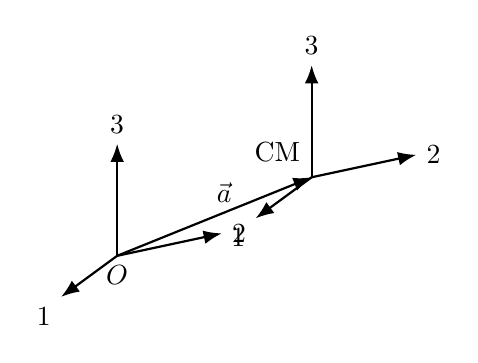
\begin{tikzpicture}[scale=0.95,>=Latex]
\draw[->,thick] (0,0) -- (0,1.5) node[above] {$3$};
\draw[->,thick] (0,0) -- (1.4,0.3) node[right] {$2$};
\draw[->,thick] (0,0) -- (-0.75,-0.55) node[below left] {$1$};
\node[below] at (0,0) {$O$};
\draw[->,thick] (0,0) -- (2.6,1.05) node[pos=0.55,above] {$\vec a$};
\begin{scope}[xshift=2.6cm,yshift=1.05cm]
\draw[->,thick] (0,0) -- (0,1.5) node[above] {$3$};
\draw[->,thick] (0,0) -- (1.4,0.3) node[right] {$2$};
\draw[->,thick] (0,0) -- (-0.75,-0.55) node[below left] {$1$};
\node[above left=1pt] at (0,0.05) {CM};
\end{scope}
\end{tikzpicture}
\caption{Two parallel triads, one at an arbitrary origin $O$ and one at the center of mass, separated by the constant vector $\vec a$; $\bar I_{ij}$ is computed about the CM triad and $I_{ij}$ about the triad at $O$.}
\label{fig:parallel-tensor}
\end{figure}

Now consider rotation with respect to an arbitrarily moving point, i.e., no longer a point fixed in space. Three frames are in play: the inertial frame; the CM frame (origin at $\vec R$, axes parallel to the inertial axes, possibly accelerated but always parallel to the inertial frame — ``translated but not rotated''); and the body frame (origin at $\vec R$, axes rotating with the body, so it is non-inertial even if $\ddot{\vec R}=\vec 0$). Figure~\ref{fig:moving-point} shows the geometry: $\vec r=\vec R+\vec r'$, with $\vec r'$ the position relative to the center of mass.

\begin{figure}[htb]
\centering
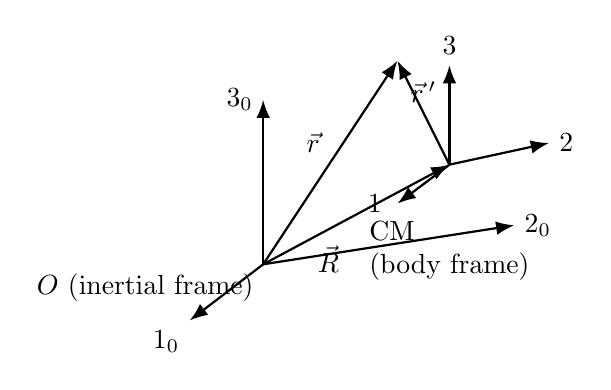
\begin{tikzpicture}[scale=1.1,>=Latex]
\draw[->,thick] (0,0) -- (0,1.9) node[left] {$3_0$};
\draw[->,thick] (0,0) -- (2.9,0.45) node[right] {$2_0$};
\draw[->,thick] (0,0) -- (-0.85,-0.65) node[below left] {$1_0$};
\node[below left] at (0,0) {$O$ (inertial frame)};
\coordinate (CM) at (2.15,1.15);
\coordinate (Pt) at (1.55,2.35);
\draw[->,thick] (0,0) -- (CM) node[pos=0.35,below=2pt] {$\vec R$};
\draw[->,thick] (0,0) -- (Pt) node[midway,above left] {$\vec r$};
\draw[->,thick] (CM) -- (Pt) node[midway,above] {$\vec r\,'$};
\begin{scope}[shift={(CM)}]
\draw[->,thick] (0,0) -- (0,1.15) node[above] {$3$};
\draw[->,thick] (0,0) -- (1.15,0.25) node[right] {$2$};
\draw[->,thick] (0,0) -- (-0.6,-0.45) node[left=2pt] {$1$};
\node[align=left] at (0,-1.0) {CM\\(body frame)};
\end{scope}
\end{tikzpicture}
\caption{Position vector $\vec r$ from the inertial origin, resolved as $\vec r=\vec R+\vec r\,'$ with $\vec R$ the center-of-mass position and $\vec r\,'$ measured from the center of mass in the (rotating) body frame.}
\label{fig:moving-point}
\end{figure}

Applying the transport theorem, Eq.~\eqref{eq:transport}, to $\vec r=\vec R+\vec r\,'$,
\begin{equation}
\left.\ddt{\vec r}\right|_{\mathrm{inertial}} = \ddt{\vec R}+\left.\ddt{\vec r\,'}\right|_{\mathrm{CM}}, \qquad
\boxed{\left.\ddt{\vec r}\right|_{\mathrm{inertial}} = \ddt{\vec R}+\left.\ddt{\vec r\,'}\right|_{\mathrm{body}}+\vec\omega\times\vec r\,',}
\label{eq:transport-r}
\end{equation}
and, since $\vec r\,'$ is constant in the body frame for a rigid body,
\begin{equation}
\boxed{\text{if rigid body:}\quad \left.\ddt{\vec r}\right|_{\mathrm{inertial}} = \ddt{\vec R}+\vec\omega\times\vec r\,'.}
\label{eq:transport-rigid}
\end{equation}
For any system of particles, with $M=\sum_P m_P$ and $\vec R\equiv\sum_P m_P\vec r_P/\sum_P m_P$ the center-of-mass position,
\begin{equation}
T = \frac12 M\dot{\vec R}^2+T', \qquad T'=\sum_P\frac{m_P}{2}\dot{\vec r}_P'^{\,2}, \qquad
\vec L^0 = \vec R\times M\dot{\vec R}+\vec L', \qquad \vec L'=\sum_P \vec r_P'\times m_P\dot{\vec r}_P',
\label{eq:general-split}
\end{equation}
where $T'$ and $\vec L'$ are measured in the frame with origin at the center of mass (the CM frame). For a rigid body, $\dot{\vec r}_P'=\vec\omega\times\vec r_P'$, so that
\begin{equation}
\vec L^0 = \vec R\times M\dot{\vec R}+\underbrace{\sum_P \vec r_P'\times m_P(\vec\omega\times\vec r_P')}_{\text{computed above}}, \qquad
T = \frac12 M\left|\dot{\vec R}\right|^2+\underbrace{\sum_P\frac{m_P}{2}\left(\vec\omega\times\vec r_P'\right)^2}_{\text{computed above}},
\label{eq:general-rigid-split}
\end{equation}
with $L_i'=\sum_j \bar I_{ij}\omega_j$ and $T'=\frac12\sum_{ij}\bar I_{ij}\omega_i\omega_j$, exactly as in Eqs.~\eqref{eq:inertia-tensor-def}--\eqref{eq:L-T-boxed} but with the inertia tensor now understood as the tensor with respect to the center of mass, $\bar I_{ij}$.

\section{Euler's Equations}

Working in the CM frame ($\vec R$ possibly accelerated but always parallel to the inertial frame — translated but not rotated), Eq.~\eqref{eq:dLdt-Ne} together with the transport theorem, Eq.~\eqref{eq:transport}, gives
\begin{equation}
\vec N = \ddt{\vec L} = \left.\ddt{\vec L}\right|_{\mathrm{body}}+\vec\omega\times\vec L,
\label{eq:N-transport}
\end{equation}
so that, component by component,
\begin{equation}
N_1 = \left.\dd{L_1}{t}\right|_{\mathrm{body}}+(\vec\omega\times\vec L)_1 = \left.\dd{L_1}{t}\right|_{\mathrm{body}}+\omega_2L_3-\omega_3L_2.
\label{eq:N1}
\end{equation}
In the principal-axis basis $L_i=I_i\omega_i$, and since a rigid body has $\dot{\vec r}_P=\vec 0$ in the body frame, $\dd{I_i}{t}\Big|_{\mathrm{body}}=0$, so
\begin{equation}
N_1 = I_1\left.\dd{\omega_1}{t}\right|_{\mathrm{body}}+\omega_2I_3\omega_3-\omega_3I_2\omega_2 = I_1\left.\dd{\omega_1}{t}\right|_{\mathrm{body}}+\omega_2\omega_3(I_3-I_2),
\label{eq:N1-final}
\end{equation}
and cyclically. Euler's equations are
\begin{equation}
\boxed{\begin{aligned}
I_1\left.\dd{\omega_1}{t}\right|_{\mathrm{body}} &= \omega_2\omega_3(I_2-I_3)+N_1,\\
I_2\left.\dd{\omega_2}{t}\right|_{\mathrm{body}} &= \omega_3\omega_1(I_3-I_1)+N_2,\\
I_3\left.\dd{\omega_3}{t}\right|_{\mathrm{body}} &= \omega_1\omega_2(I_1-I_2)+N_3.
\end{aligned}}
\label{eq:euler-eqns}
\end{equation}

\section{Application: Kater's Reversible Pendulum}

Consider a rigid pendulum with one degree of freedom, so that a single angle $\Phi$ serves as the generalized coordinate, free of friction, with body axes $\hat e_1,\hat e_2,\hat e_3$ fixed at the pivot (Fig.~\ref{fig:katers}). In the lab frame, $\omega_3=\dot\Phi$, and
\begin{equation}
I\dot\omega_3 = \dd{L_3}{t} = N_3 = -Mgl\sin\Phi,
\label{eq:kater-N3}
\end{equation}
since, with $\vec g=g(\cos\Phi\,\hat e_1-\sin\Phi\,\hat e_2)$,
\begin{equation}
\vec N_g = l\hat e_1\times M\vec g = l\hat e_1\times Mg(\cos\Phi\,\hat e_1-\sin\Phi\,\hat e_2) = -Mgl\sin\Phi\,\hat e_3,
\label{eq:kater-torque}
\end{equation}
using $\hat e_1\times\hat e_1=0$ and $\hat e_1\times\hat e_2=\hat e_3$. For small angles, $\sin\Phi\approx\Phi$, and
\begin{equation}
I\ddot\Phi \approx -Mgl\Phi, \qquad \ddot\Phi\approx-\frac{Mgl}{I}\Phi, \qquad \ddot\Phi=-\Om^2\Phi, \qquad \Om=\left(\frac{Mgl}{I}\right)^{1/2} \quad \text{(frequency of oscillation).}
\label{eq:kater-freq}
\end{equation}

\begin{figure}[htb]
\centering
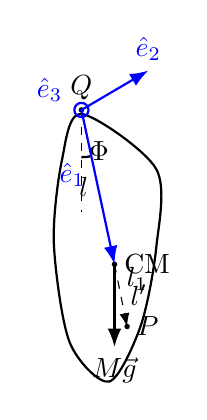
\begin{tikzpicture}[scale=1.0,>=Latex]
\coordinate (Q) at (0,4.3);
\coordinate (CM) at (0.42,2.34);
\coordinate (P) at (0.58,1.55);
% vertical reference (direction of g) and angle Phi
\draw[dashed] (Q) -- ++(0,-1.3);
\draw[thick] ($(Q)+(0,-0.6)$) arc (-90:-77.5:0.6);
\node at (0.22,3.78) {$\Phi$};
% pendulum body: elongated blob enclosing the Q-CM-P axis
\draw[thick] plot[smooth cycle] coordinates
 {(0,4.25) (0.95,3.55) (0.95,2.55) (0.75,1.55) (0.35,0.85) (-0.15,1.35) (-0.35,2.6) (-0.25,3.65)};
% pivot, CM, percussion center
\fill (Q) circle (0.035);
\node[above] at (Q) {$Q$};
\fill (CM) circle (0.035);
\node[right] at (CM) {CM};
\fill (P) circle (0.035);
\node[right] at (P) {$P$};
% body axes at the pivot
\draw[thick,blue,->] (Q) -- (CM) node[pos=0.42,left] {$\hat e_1$};
\draw[thick,blue,->] (Q) -- ++(0.85,0.5) node[above,blue] {$\hat e_2$};
\draw[thick,blue] (Q) circle (0.09);
\fill[blue] (Q) circle (0.02);
\node[above left,blue] at ($(Q)+(-0.12,-0.02)$) {$\hat e_3$};
% distances
\draw[dashed,->] (CM) -- (P) node[midway,right] {$l'$};
\node[left] at ($(Q)!0.5!(CM)$) {$l$};
\node[right] at ($(Q)!0.78!(P)$) {$l_1$};
% weight
\draw[->,thick] (CM) -- ++(0,-1.05) node[below] {$M\vec g$};
\end{tikzpicture}
\caption{Kater's reversible pendulum: body axes $\hat e_1,\hat e_2,\hat e_3$ fixed at the pivot $Q$, center of mass a distance $l$ from $Q$, percussion center $P$ a distance $l_1$ from $Q$ along the line through the center of mass, and generalized coordinate $\Phi$ measured from the vertical.}
\label{fig:katers}
\end{figure}

\subsection{Radius of Gyration and Reversibility}

Define the radius of gyration $\bar k$ about the center of mass by $\bar I\equiv M\bar k^2$, and the radius of gyration $k$ about $Q$ by $I\equiv Mk^2$; the parallel-axis theorem $I=\bar I+Ml^2$ then gives $k^2=\bar k^2+l^2$. Then
\begin{equation}
\Om_Q^2 = \frac{Mgl}{M(\bar k^2+l^2)} = \frac{g}{l_1}, \qquad l_1\equiv\frac{k^2}{l}=l+\frac{\bar k^2}{l},
\label{eq:kater-l1}
\end{equation}
with $\Om_Q$ having units of inverse time, as required, since $g/l_1$ has units of acceleration over length. Comparing with the simple pendulum (point mass, length $l$), for which $\Om=\sqrt{g/l}$: since a point mass has $\bar I=0\Rightarrow\bar k=0$, indeed $l_1=l+\bar k^2/l=l$, recovering the simple-pendulum result.

More generally,
\begin{equation}
\bar I = \int d^3r\,\rho(\vec r)\,(r_1^2+r_2^2), \qquad \bar k^2 = \frac{\bar I}{M} = \frac{\int d^3r\,\rho(\vec r)(r_1^2+r_2^2)}{\int d^3r\,\rho(\vec r)},
\label{eq:kater-Ibar}
\end{equation}
i.e., the mean-square distance to the rotation axis weighted by the mass density $\rho(\vec r)$,
with $r_1,r_2$ measured relative to the center of mass. Suspend the pendulum instead from the percussion center $P$, at distance $l_1$ from $Q$ along the direction through the center of mass; then
\begin{equation}
\Om_P^2 = \frac{gl'}{\bar k^2+l'^2} = \frac{g(l_1-l)}{\bar k^2+(l_1-l)^2} = \frac{g\,\bar k^2/l}{\bar k^2+\bar k^4/l^2} = \frac{gl}{l^2+\bar k^2} = \Om_Q^2,
\label{eq:kater-reversal}
\end{equation}
using $l_1=l+\bar k^2/l\Rightarrow l_1-l=\bar k^2/l\Rightarrow(l_1-l)^2=\bar k^4/l^2$. The oscillation frequency is thus identical whether the pendulum is suspended from $Q$ or from the percussion center $P$ a distance $l_1$ away — the basis of Kater's method for measuring $g$.

\section{Torque-Free Motion of a Symmetric Top}

For torque-free motion of a symmetric top, $I_1=I_2\neq I_3$, Euler's equations~\eqref{eq:euler-eqns} with $N_i=0$ reduce to
\begin{align}
I_1\dd{\omega_1}{t}\Big|_{\mathrm{body}} &= \omega_2\omega_3(I_2-I_3) \;\Rightarrow\; \dot\omega_1 = -\left[\omega_3\frac{I_3-I_2}{I_1}\right]\omega_2, \label{eq:sym-top-euler-1}\\
I_2\dd{\omega_2}{t}\Big|_{\mathrm{body}} &= \omega_3\omega_1(I_3-I_1) \;\Rightarrow\; \dot\omega_2 = \left[\omega_3\frac{I_3-I_1}{I_2}\right]\omega_1,
\label{eq:sym-top-euler}
\end{align}
and $I_3\dot\omega_3=\omega_1\omega_2(I_1-I_2)=0$. Defining the precession rate
\begin{equation}
\Om \equiv \omega_3\frac{I_3-I_1}{I_1},
\label{eq:precession-def}
\end{equation}
and using $I_1=I_2$,
\begin{equation}
\boxed{\dot\omega_1 = -\Om\,\omega_2,} \qquad \boxed{\dot\omega_2 = \Om\,\omega_1,} \qquad \boxed{\dot\omega_3=0.}
\label{eq:sym-top-boxed}
\end{equation}

\subsection{Precession}

Equations~\eqref{eq:sym-top-boxed} are equivalent to
\begin{equation}
\dot{\vec\omega} = \Om\hat e_3\times\vec\omega \;\iff\; \vec\omega \text{ rotates with angular velocity } \Om\hat e_3 \;\Rightarrow\; \text{precession},
\label{eq:omega-precesses}
\end{equation}
since
\begin{equation}
\dot{\vec\omega} = \Om\hat e_3\times\vec\omega = \Om\hat e_3\times(\omega_1\hat e_1+\omega_2\hat e_2+\omega_3\hat e_3) = \Om(\omega_1\hat e_2-\omega_2\hat e_1),
\label{eq:omega-precesses-expand}
\end{equation}
which reproduces $\dot\omega_1=-\Om\omega_2$, $\dot\omega_2=\Om\omega_1$, $\dot\omega_3=0$: $\vec\omega$ rotates about $\hat e_3$ with angular speed $\Om$, sweeping out the precession cone of Fig.~\ref{fig:precession-cone}. If initially $\vec\omega=\omega(\sin\lambda\,\hat e_1+\cos\lambda\,\hat e_3)$, so that $\vec\omega$ lies in the plane of $\hat e_1$ and $\hat e_3$, then
\begin{equation}
\boxed{\omega_1=\omega\sin\lambda\cos(\Om t),} \qquad \boxed{\omega_2=\omega\sin\lambda\sin(\Om t),} \qquad \boxed{\omega_3=\omega\cos\lambda.}
\label{eq:precession-solution}
\end{equation}

\begin{figure}[htb]
\centering
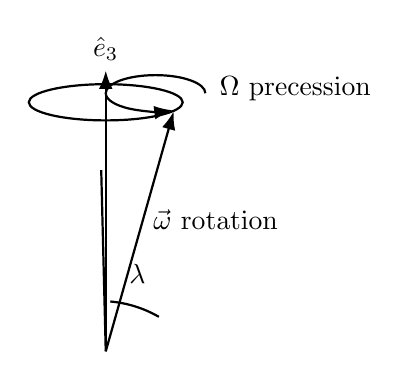
\begin{tikzpicture}[scale=1.15,>=Latex]
\draw[->,thick] (0,0) -- (0,3.1) node[above] {$\hat e_3$};
\draw[thick] (0,2.75) ellipse (0.85 and 0.2);
\draw[->,thick] (1.1,2.85) arc (0:290:0.55 and 0.2);
\node[right] at (1.15,2.9) {$\Om$ precession};
\draw[->,thick] (0,0) -- (0.75,2.65) node[pos=0.55,right] {$\vec\omega$ rotation};
\draw[thick] (0,0) -- (-0.05,2.0);
\draw[thick] (0.05,0.55) arc (85:60:1.3);
\node at (0.35,0.85) {$\lambda$};
\end{tikzpicture}
\caption{Torque-free precession of a symmetric top: the angular velocity $\vec\omega$ makes a constant angle $\lambda$ with the body symmetry axis $\hat e_3$ and sweeps out a cone at the precession rate $\Om$.}
\label{fig:precession-cone}
\end{figure}

\section{Euler Angles}

Let $\hat e_1^0,\hat e_2^0,\hat e_3^0$ be the inertial set of unit vectors (not rotating) and $\hat e_1,\hat e_2,\hat e_3$ the body set of unit vectors (rotating with the body). Six coordinates are needed to describe the positions of all points in a rigid body: the center-of-mass position $\vec R\leftrightarrow(X,Y,Z)$, and three coordinates to fix the orientation of $\hat e_1,\hat e_2,\hat e_3$ with respect to $\hat e_1^0,\hat e_2^0,\hat e_3^0$. These orientation coordinates are chosen to be the Euler angles $\alpha,\beta,\gamma$:
\begin{itemize}
\item $\ebeta\perp\hat e_3^0,\hat e_3$;
\item $\beta$ is the polar angle and $\alpha$ the azimuthal angle orienting the new ``north pole'' $\hat e_3$ relative to $\hat e_3^0$;
\item $\gamma$ specifies the additional rotation about $\hat e_3$;
\item $\alpha,\beta,\gamma$ can be chosen independently and completely specify the orientation of the body frame $\Rightarrow$ use $\alpha,\beta,\gamma$ as generalized coordinates.
\end{itemize}
Following Chapter 5 of Fetter and Walecka (skipping a considerable amount of intervening development), the kinetic energy and angular velocity are
\begin{equation}
T = \frac12\left(I_1\omega_1^2+I_2\omega_2^2+I_3\omega_3^2\right), \qquad
\vec\omega = \dot\alpha\,\hat e_3^0+\dot\beta\,\ebeta+\dot\gamma\,\hat e_3, \qquad \ebeta = \cos\gamma\,\hat e_2+\sin\gamma\,\hat e_1,
\label{eq:euler-omega-def}
\end{equation}
\begin{equation}
\hat e_3^0 = \cos\beta\,\hat e_3+\sin\beta\big[\cos\gamma\,(-\hat e_1)+\sin\gamma\,\hat e_2\big],
\label{eq:e3zero-decomp}
\end{equation}
\begin{equation}
\boxed{\vec\omega = \big(-\dot\alpha\sin\beta\cos\gamma+\dot\beta\sin\gamma\big)\hat e_1 + \big(\dot\alpha\sin\beta\sin\gamma+\dot\beta\cos\gamma\big)\hat e_2 + \big(\dot\gamma+\dot\alpha\cos\beta\big)\hat e_3.}
\label{eq:omega-euler}
\end{equation}

\begin{figure}[htb]
\centering
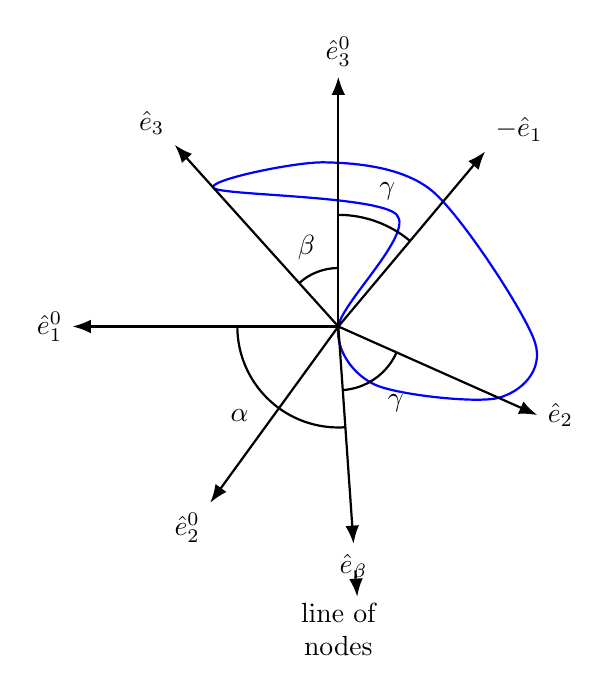
\begin{tikzpicture}[scale=1.35,>=Latex]
\coordinate (O) at (0,0);
% rays
\coordinate (e3z) at (90:2.35);
\coordinate (e3) at (132:2.3);
\coordinate (me1) at (50:2.15);
\coordinate (e1z) at (180:2.5);
\coordinate (e2z) at (234:2.05);
\coordinate (ebeta) at (274:2.05);
\coordinate (e2) at (336:2.05);
% blue tilted-plane loop (edge-on view of the e1-e2 plane)
\draw[blue,thick] plot[smooth cycle] coordinates {(0,0) (0.55,1.05) (132:1.75) (95:1.55) (55:1.55) (1.85,-0.15) (336:1.65) (0.35,-0.55)};
% rays on top
\draw[->,thick] (O) -- (e3z) node[above] {$\hat e_3^0$};
\draw[->,thick] (O) -- (e3) node[above left] {$\hat e_3$};
\draw[->,thick] (O) -- (me1) node[above right] {$-\hat e_1$};
\draw[->,thick] (O) -- (e1z) node[left] {$\hat e_1^0$};
\draw[->,thick] (O) -- (e2z) node[below left] {$\hat e_2^0$};
\draw[->,thick] (O) -- (ebeta) node[below] {$\hat e_\beta$};
\draw[->,thick] (O) -- (e2) node[right] {$\hat e_2$};
% angle arcs
\draw[thick] (90:0.55) arc (90:132:0.55);
\node at (112:0.8) {$\beta$};
\draw[thick] (90:1.05) arc (90:50:1.05);
\node at (70:1.35) {$\gamma$};
\draw[thick] (180:0.95) arc (180:274:0.95);
\node at (222:1.25) {$\alpha$};
\draw[thick] (274:0.6) arc (274:336:0.6);
\node at (307:0.9) {$\gamma$};
% line of nodes label
\draw[->,thick,dashed] (274:2.3) -- (274:2.55);
\node[align=center] at (270:2.85) {line of\\ nodes};
\end{tikzpicture}
\caption{The Euler angles $\alpha$ (azimuthal), $\beta$ (polar), $\gamma$ (spin about $\hat e_3$) relating the inertial triad $\hat e_1^0,\hat e_2^0,\hat e_3^0$ to the body triad $\hat e_1,\hat e_2,\hat e_3$. The line of nodes is the intersection of the $\hat e_1^0$-$\hat e_2^0$ and $\hat e_1$-$\hat e_2$ planes and carries the unit vector $\hat e_\beta$; the blue curve traces the (edge-on) body equatorial plane spanned by $\hat e_1,\hat e_2$.}
\label{fig:euler-angles}
\end{figure}

\subsection{Infinitesimal Rotations Add}

For infinitesimal rotations, $R_\alpha=\mathbf{1}+M_\alpha\dot\alpha\,dt$ and $R_\beta=\mathbf{1}+M_\beta\dot\beta\,dt$, so that, to order $dt$,
\begin{equation}
R_\alpha R_\beta = \mathbf{1}+(M_\alpha\dot\alpha+M_\beta\dot\beta)dt+\mathcal O(dt^2), \qquad
R_\beta R_\alpha = \mathbf{1}+(M_\beta\dot\beta+M_\alpha\dot\alpha)dt+\mathcal O(dt^2),
\label{eq:infinitesimal-comm}
\end{equation}
which are equal to order $dt$; hence infinitesimal rotations add,
\begin{equation}
\vec\omega = \vec\omega_\alpha+\vec\omega_\beta+\vec\omega_\gamma,
\label{eq:omega-add}
\end{equation}
consistent with Eq.~\eqref{eq:euler-omega-def}.

\section{Kinetic Energy in Euler Angles; the Symmetric-Top Lagrangian}

Substituting Eq.~\eqref{eq:omega-euler} into $T=\frac12(I_1\omega_1^2+I_2\omega_2^2+I_3\omega_3^2)$,
\begin{equation}
T = \frac{I_1}{2}\big(-\dot\alpha\sin\beta\cos\gamma+\dot\beta\sin\gamma\big)^2 + \frac{I_2}{2}\big(\dot\alpha\sin\beta\sin\gamma+\dot\beta\cos\gamma\big)^2 + \frac{I_3}{2}\big(\dot\gamma+\dot\alpha\cos\beta\big)^2.
\label{eq:T-euler-general}
\end{equation}
For a symmetric top, $I_1=I_2$, this simplifies to
\begin{equation}
T = \frac{I_1}{2}\big(\dot\beta^2+\dot\alpha^2\sin^2\beta\big)+\frac{I_3}{2}\big(\dot\gamma+\dot\alpha\cos\beta\big)^2,
\label{eq:T-symtop}
\end{equation}
and, since there is no potential energy contribution to the orientation coordinates for torque-free motion, the Lagrangian is
\begin{equation}
L = T = \frac{I_1}{2}\big(\dot\beta^2+\dot\alpha^2\sin^2\beta\big)+\frac{I_3}{2}\big(\dot\gamma+\dot\alpha\cos\beta\big)^2.
\label{eq:L-symtop}
\end{equation}
With generalized coordinates $\alpha,\beta,\gamma$, there are three Lagrange equations; $\alpha$ and $\gamma$ are cyclic (absent from $L$), giving two conserved momenta:
\begin{equation}
p_\alpha = \pd{L}{\dot\alpha} = I_1\sin^2\beta\,\dot\alpha + I_3(\dot\gamma+\dot\alpha\cos\beta)\cos\beta, \qquad
p_\gamma = \pd{L}{\dot\gamma} = I_3(\dot\gamma+\dot\alpha\cos\beta).
\label{eq:p-alpha-gamma}
\end{equation}
It will be shown below that $p_\alpha=\vec L\cdot\hat e_3^0$ and $p_\gamma=\vec L\cdot\hat e_3$.

\subsection{\texorpdfstring{Verifying $p_\gamma=\vec L\cdot\hat e_3$}{Verifying p\_gamma = L . e3}}

Since $p_\gamma=I_3(\dot\gamma+\dot\alpha\cos\beta)=I_3\omega_3$ by Eq.~\eqref{eq:omega-euler}, and, using
\begin{equation}
\vec L = I_1(\omega_1\hat e_1+\omega_2\hat e_2)+I_3\omega_3\hat e_3,
\label{eq:L-symtop-vec}
\end{equation}
one has immediately $\vec L\cdot\hat e_3=I_3\omega_3=p_\gamma$, as anticipated.

\subsection{\texorpdfstring{Verifying $p_\alpha=\vec L\cdot\hat e_3^0$}{Verifying p\_alpha = L . e3\^{}0}}

Compare $p_\alpha=I_1\sin^2\beta\,\dot\alpha+I_3(\dot\gamma+\dot\alpha\cos\beta)\cos\beta$ with
\begin{equation}
\vec L\cdot\hat e_3^0 = \Big(I_1(\omega_1\hat e_1+\omega_2\hat e_2)+I_3\omega_3\hat e_3\Big)\cdot\Big(\cos\beta\,\hat e_3+\sin\beta\big[\cos\gamma\,(-\hat e_1)+\sin\gamma\,\hat e_2\big]\Big),
\label{eq:L-dot-e3zero}
\end{equation}
using Eq.~\eqref{eq:e3zero-decomp}. Expanding,
\begin{align}
\vec L\cdot\hat e_3^0 &= I_1\Big[(-\dot\alpha\sin\beta\cos\gamma+\dot\beta\sin\gamma)(-\sin\beta\cos\gamma)\notag\\
&\qquad\qquad+(\dot\alpha\sin\beta\sin\gamma+\dot\beta\cos\gamma)(\sin\beta\sin\gamma)\Big] + I_3(\dot\gamma+\dot\alpha\cos\beta)\cos\beta\notag\\
&= I_1\dot\alpha\sin^2\beta\big(\cos^2\gamma+\sin^2\gamma\big) + I_3(\dot\gamma+\dot\alpha\cos\beta)\cos\beta,
\label{eq:L-dot-e3zero-expand}
\end{align}
so that
\begin{equation}
\boxed{\vec L\cdot\hat e_3^0 = I_1\dot\alpha\sin^2\beta+I_3(\dot\gamma+\dot\alpha\cos\beta)\cos\beta = p_\alpha,} \qquad \checkmark
\label{eq:palpha-verified}
\end{equation}
matching Eq.~\eqref{eq:p-alpha-gamma}.

\subsection{\texorpdfstring{The Momentum Conjugate to $\beta$}{The Momentum Conjugate to beta}}

Since $\beta$ appears explicitly in the Lagrangian, $p_\beta\equiv\pd{L}{\dot\beta}=I_1\dot\beta$ is not, in principle, a constant of the motion. Its time derivative follows from
\begin{equation}
\pd{L}{\beta} = I_1\sin\beta\cos\beta\,\dot\alpha^2 - I_3(\dot\gamma+\dot\alpha\cos\beta)\dot\alpha\sin\beta = \dot\alpha\sin\beta\big(I_1\dot\alpha\cos\beta-I_3\omega_3\big),
\label{eq:dLdbeta}
\end{equation}
so that, by the Euler-Lagrange equation,
\begin{equation}
\dot p_\beta = \pd{L}{\beta} = \dot\alpha\sin\beta\big(I_1\dot\alpha\cos\beta-I_3\omega_3\big) \qquad (\text{however, see below}).
\label{eq:pbetadot}
\end{equation}
Comparing $p_\beta=I_1\dot\beta$ with
\begin{align}
\vec L\cdot\ebeta &= \Big(I_1(\omega_1\hat e_1+\omega_2\hat e_2)+I_3\omega_3\hat e_3\Big)\cdot\big(\cos\gamma\,\hat e_2+\sin\gamma\,\hat e_1\big)\notag\\
&= I_1\Big[(-\dot\alpha\sin\beta\cos\gamma+\dot\beta\sin\gamma)\sin\gamma+(\dot\alpha\sin\beta\sin\gamma+\dot\beta\cos\gamma)\cos\gamma\Big],
\label{eq:L-dot-ebeta}
\end{align}
using Eq.~\eqref{eq:euler-omega-def}, gives
\begin{equation}
\vec L\cdot\ebeta = I_1\dot\beta\big(\sin^2\gamma+\cos^2\gamma\big) = I_1\dot\beta \;\Rightarrow\; \boxed{\vec L\cdot\ebeta = p_\beta.} \qquad\checkmark
\label{eq:pbeta-verified}
\end{equation}

\section{Description in the Inertial (or CM) Frame}

Since there is no torque, $\dot{\vec L}=\vec 0$. Choose the inertial $\hat e_3^0$ axis along the (fixed) direction of $\vec L$, so that $\vec L\cdot\hat e_3^0=|\vec L|$ and $\vec L=|\vec L|\,\hat e_3^0$; the magnitude $|\vec L|$ does not change. Since $\vec L\cdot\hat e_3=p_\gamma$ is a constant of the motion,
\begin{equation}
\vec L\cdot\hat e_3 = |\vec L|\,\hat e_3^0\cdot\hat e_3 \;\Rightarrow\; \hat e_3^0\cdot\hat e_3 = \frac{p_\gamma}{|\vec L|} = \text{const},
\label{eq:e3-e3zero-const}
\end{equation}
and since $\hat e_3^0\cdot\hat e_3=\cos(\text{angle between }\hat e_3\text{ and }\hat e_3^0)=\cos\beta$, $\beta$ is a constant of the motion:
\begin{equation}
\beta = \text{const} \;\Rightarrow\; \dot\beta=0 \;\Rightarrow\; p_\beta = I_1\dot\beta = \vec L\cdot\ebeta = 0,
\label{eq:beta-const}
\end{equation}
i.e., for this particular choice of axes, both $p_\beta$ and $\vec L\cdot\ebeta$ vanish. Since $\vec L\cdot\ebeta=0$ and $\vec L\neq\vec 0$, $|\ebeta|=1\neq0$, so
\begin{equation}
\vec L\perp\ebeta \;\Rightarrow\; \vec L \text{ lies in the plane of } \hat e_3 \text{ and } \hat e_3^0.
\label{eq:L-in-plane}
\end{equation}
The constants of the motion are $I_1,I_3,\beta,I_3\omega_3=L_3,p_\alpha$. From Eq.~\eqref{eq:p-alpha-gamma},
\begin{equation}
p_\alpha = I_1\sin^2\beta\,\dot\alpha+I_3\omega_3\cos\beta = \text{const} \;\Rightarrow\; \dot\alpha=\text{const},
\label{eq:alpha-const}
\end{equation}
since $I_1,\beta,I_3\omega_3$ are all constant. Likewise, from Eq.~\eqref{eq:p-alpha-gamma}, since $I_3,p_\gamma,\dot\alpha,\beta$ are constant, $\dot\gamma=\text{const}$. Hence
\begin{equation}
\alpha=\dot\alpha_0\,t, \qquad \gamma=\dot\gamma_0\,t, \qquad \dot\alpha_0,\dot\gamma_0 \text{ constants.}
\label{eq:alpha-gamma-linear}
\end{equation}

\subsection{\texorpdfstring{Relating $\dot\gamma$ to the Precession Rate}{Relating gamma-dot to the Precession Rate}}

Setting $\dot p_\beta=0$ in Eq.~\eqref{eq:pbetadot},
\begin{equation}
0 = \dot p_\beta = \dot\alpha\sin\beta\big(I_1\dot\alpha\cos\beta-I_3\omega_3\big) \;\Rightarrow\; \dot\alpha\cos\beta = \frac{I_3\omega_3}{I_1}
\label{eq:alpha-cosbeta}
\end{equation}
(for $\sin\beta\neq0$, $\dot\alpha\neq0$). Then, from Eq.~\eqref{eq:omega-euler}, $\omega_3=\dot\gamma+\dot\alpha\cos\beta=\dot\gamma+I_3\omega_3/I_1$, so
\begin{equation}
\boxed{\dot\gamma = \omega_3\frac{I_1-I_3}{I_1} = -\Om,}
\label{eq:gammadot-Omega}
\end{equation}
with $\Om\equiv\omega_3(I_3-I_1)/I_1$ the precession rate of Eq.~\eqref{eq:precession-def}. With $\dot\beta=0$, Eq.~\eqref{eq:euler-omega-def} reduces to
\begin{equation}
\vec\omega = \dot\alpha\,\hat e_3^0+\dot\gamma\,\hat e_3 \;\Rightarrow\; \hat e_3,\hat e_3^0,\vec\omega,\vec L \text{ all lie in one plane.}
\label{eq:one-plane}
\end{equation}
Consider the two cases $I_1=I_2<I_3$ and $I_1=I_2>I_3$, with $\vec L=I_1(\omega_1\hat e_1+\omega_2\hat e_2)+I_3\omega_3\hat e_3$ as in Eq.~\eqref{eq:L-symtop-vec}.

\subsection*{Closing Remark}

The simple-pendulum equation of motion, $\ddot\theta=-\frac{g}{l}\sin\theta$, has exactly the same functional form as the equation governing the corresponding tilt angle of a symmetric top pivoted at a point (the ``thumbtack'' problem), $(\text{angle})''=-C\sin(\text{angle})$, except that the coefficient $C$ is now an unwieldy combination of the principal moments of inertia and the precession rate $\Om$, rather than the simple ratio $g/l$.

\end{document}
